\documentclass[twoside]{book}

% Packages required by doxygen
\usepackage{fixltx2e}
\usepackage{calc}
\usepackage{doxygen}
\usepackage[export]{adjustbox} % also loads graphicx
\usepackage{graphicx}
\usepackage[utf8]{inputenc}
\usepackage{makeidx}
\usepackage{multicol}
\usepackage{multirow}
\PassOptionsToPackage{warn}{textcomp}
\usepackage{textcomp}
\usepackage[nointegrals]{wasysym}
\usepackage[table]{xcolor}

% Font selection
\usepackage[T1]{fontenc}
\usepackage[scaled=.90]{helvet}
\usepackage{courier}
\usepackage{amssymb}
\usepackage{sectsty}
\renewcommand{\familydefault}{\sfdefault}
\allsectionsfont{%
  \fontseries{bc}\selectfont%
  \color{darkgray}%
}
\renewcommand{\DoxyLabelFont}{%
  \fontseries{bc}\selectfont%
  \color{darkgray}%
}
\newcommand{\+}{\discretionary{\mbox{\scriptsize$\hookleftarrow$}}{}{}}

% Page & text layout
\usepackage{geometry}
\geometry{%
  a4paper,%
  top=2.5cm,%
  bottom=2.5cm,%
  left=2.5cm,%
  right=2.5cm%
}
\tolerance=750
\hfuzz=15pt
\hbadness=750
\setlength{\emergencystretch}{15pt}
\setlength{\parindent}{0cm}
\setlength{\parskip}{3ex plus 2ex minus 2ex}
\makeatletter
\renewcommand{\paragraph}{%
  \@startsection{paragraph}{4}{0ex}{-1.0ex}{1.0ex}{%
    \normalfont\normalsize\bfseries\SS@parafont%
  }%
}
\renewcommand{\subparagraph}{%
  \@startsection{subparagraph}{5}{0ex}{-1.0ex}{1.0ex}{%
    \normalfont\normalsize\bfseries\SS@subparafont%
  }%
}
\makeatother

% Headers & footers
\usepackage{fancyhdr}
\pagestyle{fancyplain}
\fancyhead[LE]{\fancyplain{}{\bfseries\thepage}}
\fancyhead[CE]{\fancyplain{}{}}
\fancyhead[RE]{\fancyplain{}{\bfseries\leftmark}}
\fancyhead[LO]{\fancyplain{}{\bfseries\rightmark}}
\fancyhead[CO]{\fancyplain{}{}}
\fancyhead[RO]{\fancyplain{}{\bfseries\thepage}}
\fancyfoot[LE]{\fancyplain{}{}}
\fancyfoot[CE]{\fancyplain{}{}}
\fancyfoot[RE]{\fancyplain{}{\bfseries\scriptsize Generated by Doxygen }}
\fancyfoot[LO]{\fancyplain{}{\bfseries\scriptsize Generated by Doxygen }}
\fancyfoot[CO]{\fancyplain{}{}}
\fancyfoot[RO]{\fancyplain{}{}}
\renewcommand{\footrulewidth}{0.4pt}
\renewcommand{\chaptermark}[1]{%
  \markboth{#1}{}%
}
\renewcommand{\sectionmark}[1]{%
  \markright{\thesection\ #1}%
}

% Indices & bibliography
\usepackage{natbib}
\usepackage[titles]{tocloft}
\setcounter{tocdepth}{3}
\setcounter{secnumdepth}{5}
\makeindex

% Hyperlinks (required, but should be loaded last)
\usepackage{ifpdf}
\ifpdf
  \usepackage[pdftex,pagebackref=true]{hyperref}
\else
  \usepackage[ps2pdf,pagebackref=true]{hyperref}
\fi
\hypersetup{%
  colorlinks=true,%
  linkcolor=blue,%
  citecolor=blue,%
  unicode%
}

% Custom commands
\newcommand{\clearemptydoublepage}{%
  \newpage{\pagestyle{empty}\cleardoublepage}%
}

\usepackage{caption}
\captionsetup{labelsep=space,justification=centering,font={bf},singlelinecheck=off,skip=4pt,position=top}

%===== C O N T E N T S =====

\begin{document}

% Titlepage & ToC
\hypersetup{pageanchor=false,
             bookmarksnumbered=true,
             pdfencoding=unicode
            }
\pagenumbering{alph}
\begin{titlepage}
\vspace*{7cm}
\begin{center}%
{\Large P\+C\+S\+C2017-\/\+Data Approximation }\\
\vspace*{1cm}
{\large Generated by Doxygen 1.8.14}\\
\end{center}
\end{titlepage}
\clearemptydoublepage
\pagenumbering{roman}
\tableofcontents
\clearemptydoublepage
\pagenumbering{arabic}
\hypersetup{pageanchor=true}

%--- Begin generated contents ---
\chapter{P\+C\+S\+C2017\+\_\+\+Group5}
\label{md___users_davidcleres__c_lion_projects__p_c_s_c2017__group5__r_e_a_d_m_e}
\Hypertarget{md___users_davidcleres__c_lion_projects__p_c_s_c2017__group5__r_e_a_d_m_e}
This is the project for the E\+P\+FL class Programming Concepts in Scientific Computing -\/ Master 1 Class -\/ Computer Science and Engineering

The program could be use simply by importing the project repository in C\+Lion and to run the project. Once the project. was launched one has the possibility to chose between execut-\/ ing the program by using a manual input in the terminal (by hitting 1) and using the information saved in the config.\+dat file (by hitting 2). However both ways of doing lead to the same functionalities. The user could chose between five different options by simply entering a number between 1 and 5 in the C\+Lion terminal. As explicitly mentioned in the C\+Lion terminal the user could use 1. to perform a Least Squares data approximation, type 2. to appreciate the graphs of Fourier data approximation, 3. to compute the \mbox{\hyperlink{class_lagrange}{Lagrange}} polynomial data approximation, 4. for the Piece\+Wise Least Square data approximation and finally 5. for the Piece\+Wise \mbox{\hyperlink{class_lagrange}{Lagrange}} data approximation. The config.\+dat file contained four lines. The first field, labeled with Approximation Method, should contain a number between 1 and 5. In this line the user could choose between the five possible approximation techniques. More, the second field was used to specific with function the user wanted to interpolate. The third and fourth fields were not necessarily used by all the approximation methods. For instance the Fourier approximation did not need these last two lines so one could give random numbers in these containers (as long as there were some values). This was also true for the \mbox{\hyperlink{class_lagrange}{Lagrange}} approximation code. The other methods, like least Square, \mbox{\hyperlink{class_lagrange}{Lagrange}} by single pieces needed the first three lines in order to specify the degree of the polynomial function to interpolate. Finally, Least Square approximation by pieces needed all the four lines. In this specific case, all four fields were necessary since the method needed to know the degree and the number of intervals to compute. By doing all the steps as mentioned in the two previous paragraphs all the programs should work well and give a qualified approximation of the function. During the execution of the program he user had to follow the instructions on the terminal. However, it is important to know the pipeline of execution, meaning that once everything was entered the program took a few second to compute the answer. Following this step a graph appeared on the screen for 20 seconds. Once the first graph disappeared the testing part of the program was launched and showed a graph again but this time only comparing the expected data with the interpolation. This lasted for 20 seconds again and was then followed by a displaying of the accuracy of the prediction in comparison to the real data. 
\chapter{Hierarchical Index}
\section{Class Hierarchy}
This inheritance list is sorted roughly, but not completely, alphabetically\+:\begin{DoxyCompactList}
\item \contentsline{section}{Data}{\pageref{struct_data}}{}
\item \contentsline{section}{F\+F\+Treal}{\pageref{class_f_f_treal}}{}
\item \contentsline{section}{Gnuplot}{\pageref{class_gnuplot}}{}
\item \contentsline{section}{Graph}{\pageref{class_graph}}{}
\item \contentsline{section}{Lagrange}{\pageref{class_lagrange}}{}
\item \contentsline{section}{Piece\+Wise\+Continue\+Polynomial}{\pageref{class_piece_wise_continue_polynomial}}{}
\item \contentsline{section}{Point}{\pageref{class_point}}{}
\item \contentsline{section}{point\+\_\+t}{\pageref{structpoint__t}}{}
\item \contentsline{section}{Polynomial}{\pageref{class_polynomial}}{}
\item \contentsline{section}{Read\+File}{\pageref{class_read_file}}{}
\item \contentsline{section}{Reafile}{\pageref{class_reafile}}{}
\item runtime\+\_\+error\begin{DoxyCompactList}
\item \contentsline{section}{Gnuplot\+Exception}{\pageref{class_gnuplot_exception}}{}
\end{DoxyCompactList}
\end{DoxyCompactList}

\chapter{Class Index}
\section{Class List}
Here are the classes, structs, unions and interfaces with brief descriptions\+:\begin{DoxyCompactList}
\item\contentsline{section}{\mbox{\hyperlink{struct_data}{Data}} }{\pageref{struct_data}}{}
\item\contentsline{section}{\mbox{\hyperlink{class_f_f_treal}{F\+F\+Treal}} }{\pageref{class_f_f_treal}}{}
\item\contentsline{section}{\mbox{\hyperlink{class_gnuplot}{Gnuplot}} }{\pageref{class_gnuplot}}{}
\item\contentsline{section}{\mbox{\hyperlink{class_gnuplot_exception}{Gnuplot\+Exception}} }{\pageref{class_gnuplot_exception}}{}
\item\contentsline{section}{\mbox{\hyperlink{class_graph}{Graph}} }{\pageref{class_graph}}{}
\item\contentsline{section}{\mbox{\hyperlink{class_lagrange}{Lagrange}} \\*This is redefinition of the virtual class to implement \mbox{\hyperlink{class_lagrange}{Lagrange}} functions

This is how we can calculate the approximation of the data using \mbox{\hyperlink{class_lagrange}{Lagrange}} Polynome }{\pageref{class_lagrange}}{}
\item\contentsline{section}{\mbox{\hyperlink{class_piece_wise_continue_polynomial}{Piece\+Wise\+Continue\+Polynomial}} }{\pageref{class_piece_wise_continue_polynomial}}{}
\item\contentsline{section}{\mbox{\hyperlink{class_point}{Point}} }{\pageref{class_point}}{}
\item\contentsline{section}{\mbox{\hyperlink{structpoint__t}{point\+\_\+t}} }{\pageref{structpoint__t}}{}
\item\contentsline{section}{\mbox{\hyperlink{class_polynomial}{Polynomial}} }{\pageref{class_polynomial}}{}
\item\contentsline{section}{\mbox{\hyperlink{class_read_file}{Read\+File}} }{\pageref{class_read_file}}{}
\item\contentsline{section}{\mbox{\hyperlink{class_reafile}{Reafile}} \\*This is a simple positions accessor }{\pageref{class_reafile}}{}
\end{DoxyCompactList}

\chapter{File Index}
\section{File List}
Here is a list of all files with brief descriptions\+:\begin{DoxyCompactList}
\item\contentsline{section}{/\+Users/davidcleres/\+C\+Lion\+Projects/\+P\+C\+S\+C2017\+\_\+\+Group5/\mbox{\hyperlink{_abstract_numerical_approximation_8cpp}{Abstract\+Numerical\+Approximation.\+cpp}} }{\pageref{_abstract_numerical_approximation_8cpp}}{}
\item\contentsline{section}{/\+Users/davidcleres/\+C\+Lion\+Projects/\+P\+C\+S\+C2017\+\_\+\+Group5/\mbox{\hyperlink{_abstract_numerical_approximation_8h}{Abstract\+Numerical\+Approximation.\+h}} \\*This is the virtual class we will use to implement all the approximations functions This is a pure virtual class }{\pageref{_abstract_numerical_approximation_8h}}{}
\item\contentsline{section}{/\+Users/davidcleres/\+C\+Lion\+Projects/\+P\+C\+S\+C2017\+\_\+\+Group5/\mbox{\hyperlink{_f_f_treal_8cpp}{F\+F\+Treal.\+cpp}} }{\pageref{_f_f_treal_8cpp}}{}
\item\contentsline{section}{/\+Users/davidcleres/\+C\+Lion\+Projects/\+P\+C\+S\+C2017\+\_\+\+Group5/\mbox{\hyperlink{_f_f_treal_8h}{F\+F\+Treal.\+h}} }{\pageref{_f_f_treal_8h}}{}
\item\contentsline{section}{/\+Users/davidcleres/\+C\+Lion\+Projects/\+P\+C\+S\+C2017\+\_\+\+Group5/\mbox{\hyperlink{_f_f_ttest_8cpp}{F\+F\+Ttest.\+cpp}} }{\pageref{_f_f_ttest_8cpp}}{}
\item\contentsline{section}{/\+Users/davidcleres/\+C\+Lion\+Projects/\+P\+C\+S\+C2017\+\_\+\+Group5/\mbox{\hyperlink{gnuplot__i_8cpp}{gnuplot\+\_\+i.\+cpp}} \\*This is a direct translation from the C interface written by N. Devillard (which is available from \href{http://ndevilla.free.fr/gnuplot/}{\tt http\+://ndevilla.\+free.\+fr/gnuplot/}). As in the C interface this uses pipes and so wont run on a system that doesn\textquotesingle{}t have P\+O\+S\+IX pipe support }{\pageref{gnuplot__i_8cpp}}{}
\item\contentsline{section}{/\+Users/davidcleres/\+C\+Lion\+Projects/\+P\+C\+S\+C2017\+\_\+\+Group5/\mbox{\hyperlink{gnuplot__i_8hpp}{gnuplot\+\_\+i.\+hpp}} }{\pageref{gnuplot__i_8hpp}}{}
\item\contentsline{section}{/\+Users/davidcleres/\+C\+Lion\+Projects/\+P\+C\+S\+C2017\+\_\+\+Group5/\mbox{\hyperlink{_lagrange_8cpp}{Lagrange.\+cpp}} }{\pageref{_lagrange_8cpp}}{}
\item\contentsline{section}{/\+Users/davidcleres/\+C\+Lion\+Projects/\+P\+C\+S\+C2017\+\_\+\+Group5/\mbox{\hyperlink{_lagrange_8h}{Lagrange.\+h}} \\*This is redefinition of the virtual class to implement \mbox{\hyperlink{class_lagrange}{Lagrange}} functions }{\pageref{_lagrange_8h}}{}
\item\contentsline{section}{/\+Users/davidcleres/\+C\+Lion\+Projects/\+P\+C\+S\+C2017\+\_\+\+Group5/\mbox{\hyperlink{_least_square_8cpp}{Least\+Square.\+cpp}} }{\pageref{_least_square_8cpp}}{}
\item\contentsline{section}{/\+Users/davidcleres/\+C\+Lion\+Projects/\+P\+C\+S\+C2017\+\_\+\+Group5/\mbox{\hyperlink{_least_square_8h}{Least\+Square.\+h}} }{\pageref{_least_square_8h}}{}
\item\contentsline{section}{/\+Users/davidcleres/\+C\+Lion\+Projects/\+P\+C\+S\+C2017\+\_\+\+Group5/\mbox{\hyperlink{main_8cpp}{main.\+cpp}} \\*This is the function to call to run the script of the project }{\pageref{main_8cpp}}{}
\item\contentsline{section}{/\+Users/davidcleres/\+C\+Lion\+Projects/\+P\+C\+S\+C2017\+\_\+\+Group5/\mbox{\hyperlink{_piece_wise___continue___polynomial_8cpp}{Piece\+Wise\+\_\+\+Continue\+\_\+\+Polynomial.\+cpp}} }{\pageref{_piece_wise___continue___polynomial_8cpp}}{}
\item\contentsline{section}{/\+Users/davidcleres/\+C\+Lion\+Projects/\+P\+C\+S\+C2017\+\_\+\+Group5/\mbox{\hyperlink{_piece_wise___continue___polynomial_8h}{Piece\+Wise\+\_\+\+Continue\+\_\+\+Polynomial.\+h}} }{\pageref{_piece_wise___continue___polynomial_8h}}{}
\item\contentsline{section}{/\+Users/davidcleres/\+C\+Lion\+Projects/\+P\+C\+S\+C2017\+\_\+\+Group5/\mbox{\hyperlink{_piece_wise___non_continue___polynomial_8cpp}{Piece\+Wise\+\_\+\+Non\+Continue\+\_\+\+Polynomial.\+cpp}} }{\pageref{_piece_wise___non_continue___polynomial_8cpp}}{}
\item\contentsline{section}{/\+Users/davidcleres/\+C\+Lion\+Projects/\+P\+C\+S\+C2017\+\_\+\+Group5/\mbox{\hyperlink{_piece_wise___non_continue___polynomial_8h}{Piece\+Wise\+\_\+\+Non\+Continue\+\_\+\+Polynomial.\+h}} }{\pageref{_piece_wise___non_continue___polynomial_8h}}{}
\item\contentsline{section}{/\+Users/davidcleres/\+C\+Lion\+Projects/\+P\+C\+S\+C2017\+\_\+\+Group5/\mbox{\hyperlink{plots_8m}{plots.\+m}} }{\pageref{plots_8m}}{}
\item\contentsline{section}{/\+Users/davidcleres/\+C\+Lion\+Projects/\+P\+C\+S\+C2017\+\_\+\+Group5/\mbox{\hyperlink{_polynomial_8cpp}{Polynomial.\+cpp}} \\*This is the function to call to run the script of the project }{\pageref{_polynomial_8cpp}}{}
\item\contentsline{section}{/\+Users/davidcleres/\+C\+Lion\+Projects/\+P\+C\+S\+C2017\+\_\+\+Group5/\mbox{\hyperlink{_polynomial_8h}{Polynomial.\+h}} \\*This is the function to call to run the script of the project }{\pageref{_polynomial_8h}}{}
\item\contentsline{section}{/\+Users/davidcleres/\+C\+Lion\+Projects/\+P\+C\+S\+C2017\+\_\+\+Group5/\mbox{\hyperlink{read_file_8cpp}{read\+File.\+cpp}} }{\pageref{read_file_8cpp}}{}
\item\contentsline{section}{/\+Users/davidcleres/\+C\+Lion\+Projects/\+P\+C\+S\+C2017\+\_\+\+Group5/\mbox{\hyperlink{read_file_8h}{read\+File.\+h}} }{\pageref{read_file_8h}}{}
\item\contentsline{section}{/\+Users/davidcleres/\+C\+Lion\+Projects/\+P\+C\+S\+C2017\+\_\+\+Group5/\mbox{\hyperlink{simulation_8m}{simulation.\+m}} }{\pageref{simulation_8m}}{}
\item\contentsline{section}{/\+Users/davidcleres/\+C\+Lion\+Projects/\+P\+C\+S\+C2017\+\_\+\+Group5/cmake-\/build-\/debug/\+C\+Make\+Files/\mbox{\hyperlink{feature__tests_8c}{feature\+\_\+tests.\+c}} }{\pageref{feature__tests_8c}}{}
\item\contentsline{section}{/\+Users/davidcleres/\+C\+Lion\+Projects/\+P\+C\+S\+C2017\+\_\+\+Group5/cmake-\/build-\/debug/\+C\+Make\+Files/\mbox{\hyperlink{feature__tests_8cxx}{feature\+\_\+tests.\+cxx}} }{\pageref{feature__tests_8cxx}}{}
\item\contentsline{section}{/\+Users/davidcleres/\+C\+Lion\+Projects/\+P\+C\+S\+C2017\+\_\+\+Group5/cmake-\/build-\/debug/\+C\+Make\+Files/3.\+8.\+2/\+Compiler\+Id\+C/\mbox{\hyperlink{_c_make_c_compiler_id_8c}{C\+Make\+C\+Compiler\+Id.\+c}} }{\pageref{_c_make_c_compiler_id_8c}}{}
\item\contentsline{section}{/\+Users/davidcleres/\+C\+Lion\+Projects/\+P\+C\+S\+C2017\+\_\+\+Group5/cmake-\/build-\/debug/\+C\+Make\+Files/3.\+8.\+2/\+Compiler\+Id\+C\+X\+X/\mbox{\hyperlink{_c_make_c_x_x_compiler_id_8cpp}{C\+Make\+C\+X\+X\+Compiler\+Id.\+cpp}} }{\pageref{_c_make_c_x_x_compiler_id_8cpp}}{}
\end{DoxyCompactList}

\chapter{Class Documentation}
\hypertarget{class_read_file}{}\section{Read\+File Class Reference}
\label{class_read_file}\index{Read\+File@{Read\+File}}


{\ttfamily \#include $<$read\+File.\+h$>$}

\subsection*{Public Member Functions}
\begin{DoxyCompactItemize}
\item 
\mbox{\hyperlink{class_read_file_ae297f0539380fc9b703a1bceda2ce820}{Read\+File}} (std\+::string const \&filename)
\item 
void \mbox{\hyperlink{class_read_file_a232df426223b84e4dbb3f964ee4c3177}{load\+From\+File}} (\mbox{\hyperlink{struct_data}{Data}} \&data)
\item 
std\+::string \mbox{\hyperlink{class_read_file_a9835264c9ec95cfdbc1349573402fc01}{get\+Filename}} ()
\item 
void \mbox{\hyperlink{class_read_file_a5efc41b900510ae038dafc23a2563300}{show}} (\mbox{\hyperlink{struct_data}{Data}} const \&data)
\item 
void \mbox{\hyperlink{class_read_file_ac11779a3630a2c1d62ab4566abb4034a}{write\+File}} (\mbox{\hyperlink{struct_data}{Data}} const \&data)
\end{DoxyCompactItemize}


\subsection{Detailed Description}


Definition at line 32 of file read\+File.\+h.



\subsection{Constructor \& Destructor Documentation}
\mbox{\Hypertarget{class_read_file_ae297f0539380fc9b703a1bceda2ce820}\label{class_read_file_ae297f0539380fc9b703a1bceda2ce820}} 
\index{Read\+File@{Read\+File}!Read\+File@{Read\+File}}
\index{Read\+File@{Read\+File}!Read\+File@{Read\+File}}
\subsubsection{\texorpdfstring{Read\+File()}{ReadFile()}}
{\footnotesize\ttfamily Read\+File\+::\+Read\+File (\begin{DoxyParamCaption}\item[{std\+::string const \&}]{filename }\end{DoxyParamCaption})\hspace{0.3cm}{\ttfamily [explicit]}}







Definition at line 54 of file read\+File.\+cpp.



\subsection{Member Function Documentation}
\mbox{\Hypertarget{class_read_file_a9835264c9ec95cfdbc1349573402fc01}\label{class_read_file_a9835264c9ec95cfdbc1349573402fc01}} 
\index{Read\+File@{Read\+File}!get\+Filename@{get\+Filename}}
\index{get\+Filename@{get\+Filename}!Read\+File@{Read\+File}}
\subsubsection{\texorpdfstring{get\+Filename()}{getFilename()}}
{\footnotesize\ttfamily std\+::string Read\+File\+::get\+Filename (\begin{DoxyParamCaption}{ }\end{DoxyParamCaption})}







Definition at line 58 of file read\+File.\+cpp.

\mbox{\Hypertarget{class_read_file_a232df426223b84e4dbb3f964ee4c3177}\label{class_read_file_a232df426223b84e4dbb3f964ee4c3177}} 
\index{Read\+File@{Read\+File}!load\+From\+File@{load\+From\+File}}
\index{load\+From\+File@{load\+From\+File}!Read\+File@{Read\+File}}
\subsubsection{\texorpdfstring{load\+From\+File()}{loadFromFile()}}
{\footnotesize\ttfamily void Read\+File\+::load\+From\+File (\begin{DoxyParamCaption}\item[{\mbox{\hyperlink{struct_data}{Data}} \&}]{data }\end{DoxyParamCaption})}







Definition at line 13 of file read\+File.\+cpp.

\mbox{\Hypertarget{class_read_file_a5efc41b900510ae038dafc23a2563300}\label{class_read_file_a5efc41b900510ae038dafc23a2563300}} 
\index{Read\+File@{Read\+File}!show@{show}}
\index{show@{show}!Read\+File@{Read\+File}}
\subsubsection{\texorpdfstring{show()}{show()}}
{\footnotesize\ttfamily void Read\+File\+::show (\begin{DoxyParamCaption}\item[{\mbox{\hyperlink{struct_data}{Data}} const \&}]{data }\end{DoxyParamCaption})}







Definition at line 62 of file read\+File.\+cpp.

\mbox{\Hypertarget{class_read_file_ac11779a3630a2c1d62ab4566abb4034a}\label{class_read_file_ac11779a3630a2c1d62ab4566abb4034a}} 
\index{Read\+File@{Read\+File}!write\+File@{write\+File}}
\index{write\+File@{write\+File}!Read\+File@{Read\+File}}
\subsubsection{\texorpdfstring{write\+File()}{writeFile()}}
{\footnotesize\ttfamily void Read\+File\+::write\+File (\begin{DoxyParamCaption}\item[{\mbox{\hyperlink{struct_data}{Data}} const \&}]{data }\end{DoxyParamCaption})}







Definition at line 69 of file read\+File.\+cpp.



The documentation for this class was generated from the following files\+:\begin{DoxyCompactItemize}
\item 
/\+Users/davidcleres/\+C\+Lion\+Projects/\+P\+C\+S\+C2017\+\_\+\+Group5/\mbox{\hyperlink{read_file_8h}{read\+File.\+h}}\item 
/\+Users/davidcleres/\+C\+Lion\+Projects/\+P\+C\+S\+C2017\+\_\+\+Group5/\mbox{\hyperlink{read_file_8cpp}{read\+File.\+cpp}}\end{DoxyCompactItemize}

\hypertarget{class_reafile}{}\section{Reafile Class Reference}
\label{class_reafile}\index{Reafile@{Reafile}}


This is a simple positions accessor.  




{\ttfamily \#include $<$read\+File.\+h$>$}



\subsection{Detailed Description}
This is a simple positions accessor. 

The documentation for this class was generated from the following file\+:\begin{DoxyCompactItemize}
\item 
/\+Users/davidcleres/\+C\+Lion\+Projects/\+P\+C\+S\+C2017\+\_\+\+Group5/\mbox{\hyperlink{read_file_8h}{read\+File.\+h}}\end{DoxyCompactItemize}

\hypertarget{class_super_cool_class}{}\section{Super\+Cool\+Class Class Reference}
\label{class_super_cool_class}\index{Super\+Cool\+Class@{Super\+Cool\+Class}}


{\ttfamily \#include $<$super\+\_\+cool\+\_\+class.\+h$>$}

Inheritance diagram for Super\+Cool\+Class\+:\begin{figure}[H]
\begin{center}
\leavevmode
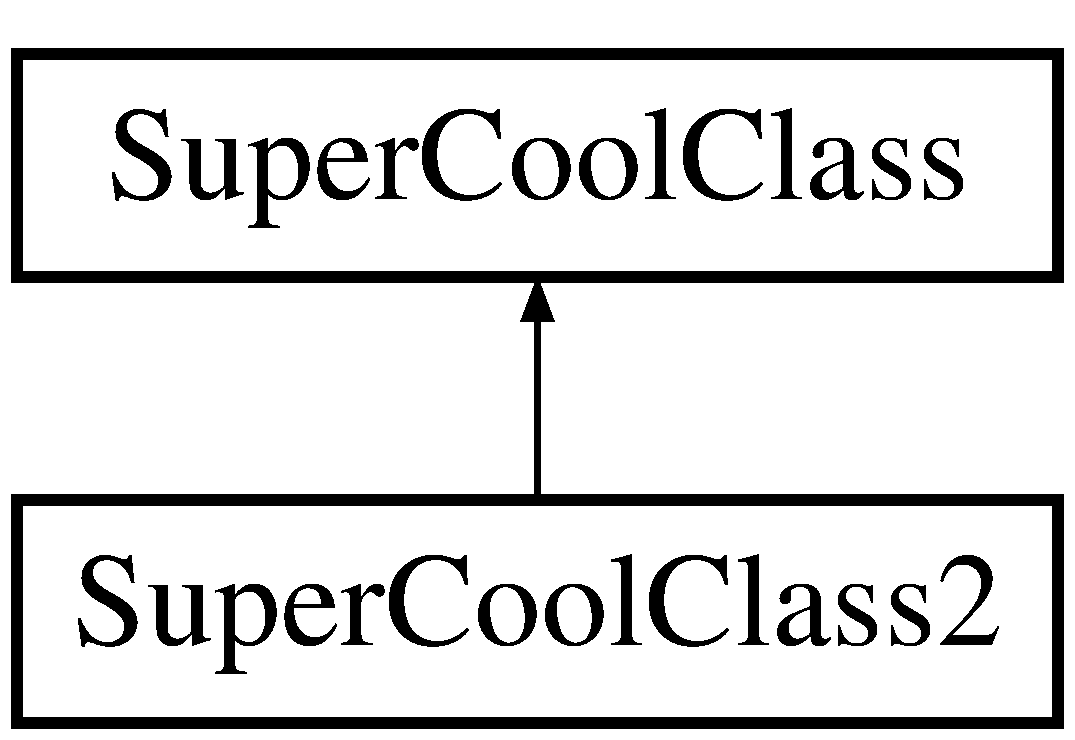
\includegraphics[height=2.000000cm]{class_super_cool_class}
\end{center}
\end{figure}
\subsection*{Public Member Functions}
\begin{DoxyCompactItemize}
\item 
\mbox{\hyperlink{struct_vector}{Vector}} \mbox{\hyperlink{class_super_cool_class_a761c470f000de1a101a855de2d49d195}{get\+Position}} (unsigned int dir)
\end{DoxyCompactItemize}
\subsection*{Protected Attributes}
\begin{DoxyCompactItemize}
\item 
int \mbox{\hyperlink{class_super_cool_class_a0264bf7dc5bfe0057907102b2b5b767d}{var}}
\end{DoxyCompactItemize}


\subsection{Detailed Description}


Definition at line 15 of file super\+\_\+cool\+\_\+class.\+h.



\subsection{Member Function Documentation}
\mbox{\Hypertarget{class_super_cool_class_a761c470f000de1a101a855de2d49d195}\label{class_super_cool_class_a761c470f000de1a101a855de2d49d195}} 
\index{Super\+Cool\+Class@{Super\+Cool\+Class}!get\+Position@{get\+Position}}
\index{get\+Position@{get\+Position}!Super\+Cool\+Class@{Super\+Cool\+Class}}
\subsubsection{\texorpdfstring{get\+Position()}{getPosition()}}
{\footnotesize\ttfamily \mbox{\hyperlink{struct_vector}{Vector}} Super\+Cool\+Class\+::get\+Position (\begin{DoxyParamCaption}\item[{unsigned int}]{dir }\end{DoxyParamCaption})\hspace{0.3cm}{\ttfamily [inline]}}



Definition at line 18 of file super\+\_\+cool\+\_\+class.\+h.



\subsection{Member Data Documentation}
\mbox{\Hypertarget{class_super_cool_class_a0264bf7dc5bfe0057907102b2b5b767d}\label{class_super_cool_class_a0264bf7dc5bfe0057907102b2b5b767d}} 
\index{Super\+Cool\+Class@{Super\+Cool\+Class}!var@{var}}
\index{var@{var}!Super\+Cool\+Class@{Super\+Cool\+Class}}
\subsubsection{\texorpdfstring{var}{var}}
{\footnotesize\ttfamily int Super\+Cool\+Class\+::var\hspace{0.3cm}{\ttfamily [protected]}}



Definition at line 20 of file super\+\_\+cool\+\_\+class.\+h.



The documentation for this class was generated from the following file\+:\begin{DoxyCompactItemize}
\item 
/\+Users/davidcleres/\+C\+Lion\+Projects/\+P\+C\+S\+C2017\+\_\+\+Group5/\mbox{\hyperlink{super__cool__class_8h}{super\+\_\+cool\+\_\+class.\+h}}\end{DoxyCompactItemize}

\hypertarget{class_super_cool_class2}{}\section{Super\+Cool\+Class2 Class Reference}
\label{class_super_cool_class2}\index{Super\+Cool\+Class2@{Super\+Cool\+Class2}}


{\ttfamily \#include $<$super\+\_\+cool\+\_\+class.\+h$>$}

Inheritance diagram for Super\+Cool\+Class2\+:\begin{figure}[H]
\begin{center}
\leavevmode
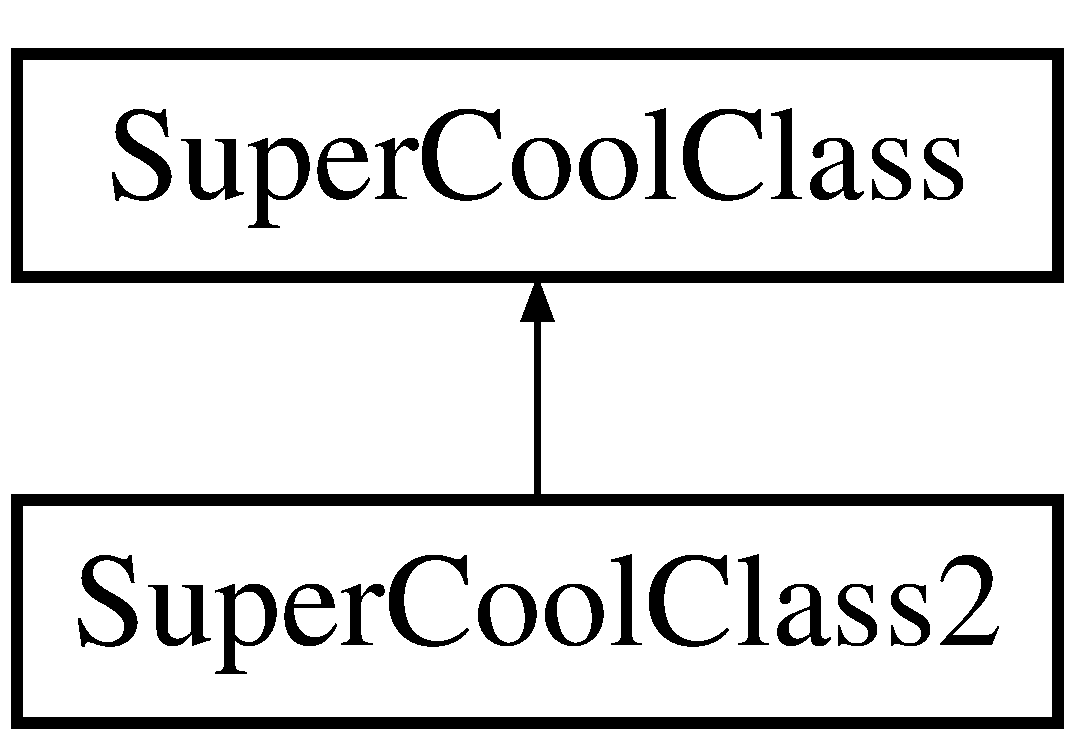
\includegraphics[height=2.000000cm]{class_super_cool_class2}
\end{center}
\end{figure}
\subsection*{Additional Inherited Members}


\subsection{Detailed Description}


Definition at line 28 of file super\+\_\+cool\+\_\+class.\+h.



The documentation for this class was generated from the following file\+:\begin{DoxyCompactItemize}
\item 
/\+Users/davidcleres/\+C\+Lion\+Projects/\+P\+C\+S\+C2017\+\_\+\+Group5/\mbox{\hyperlink{super__cool__class_8h}{super\+\_\+cool\+\_\+class.\+h}}\end{DoxyCompactItemize}

\hypertarget{struct_vector}{}\section{Vector Struct Reference}
\label{struct_vector}\index{Vector@{Vector}}


{\ttfamily \#include $<$super\+\_\+cool\+\_\+class.\+h$>$}

\subsection*{Public Attributes}
\begin{DoxyCompactItemize}
\item 
double \mbox{\hyperlink{struct_vector_adc995472c3e3bd817a76e705f2eddc90}{val}} \mbox{[}3\mbox{]}
\end{DoxyCompactItemize}


\subsection{Detailed Description}


Definition at line 9 of file super\+\_\+cool\+\_\+class.\+h.



\subsection{Member Data Documentation}
\mbox{\Hypertarget{struct_vector_adc995472c3e3bd817a76e705f2eddc90}\label{struct_vector_adc995472c3e3bd817a76e705f2eddc90}} 
\index{Vector@{Vector}!val@{val}}
\index{val@{val}!Vector@{Vector}}
\subsubsection{\texorpdfstring{val}{val}}
{\footnotesize\ttfamily double Vector\+::val\mbox{[}3\mbox{]}}



Definition at line 11 of file super\+\_\+cool\+\_\+class.\+h.



The documentation for this struct was generated from the following file\+:\begin{DoxyCompactItemize}
\item 
/\+Users/davidcleres/\+C\+Lion\+Projects/\+P\+C\+S\+C2017\+\_\+\+Group5/\mbox{\hyperlink{super__cool__class_8h}{super\+\_\+cool\+\_\+class.\+h}}\end{DoxyCompactItemize}

\chapter{File Documentation}
\hypertarget{_c_make_c_compiler_id_8c}{}\section{/\+Users/davidcleres/\+C\+Lion\+Projects/\+P\+C\+S\+C2017\+\_\+\+Group5/cmake-\/build-\/debug/\+C\+Make\+Files/3.8.2/\+Compiler\+Id\+C/\+C\+Make\+C\+Compiler\+Id.c File Reference}
\label{_c_make_c_compiler_id_8c}\index{/\+Users/davidcleres/\+C\+Lion\+Projects/\+P\+C\+S\+C2017\+\_\+\+Group5/cmake-\/build-\/debug/\+C\+Make\+Files/3.\+8.\+2/\+Compiler\+Id\+C/\+C\+Make\+C\+Compiler\+Id.\+c@{/\+Users/davidcleres/\+C\+Lion\+Projects/\+P\+C\+S\+C2017\+\_\+\+Group5/cmake-\/build-\/debug/\+C\+Make\+Files/3.\+8.\+2/\+Compiler\+Id\+C/\+C\+Make\+C\+Compiler\+Id.\+c}}
\subsection*{Macros}
\begin{DoxyCompactItemize}
\item 
\#define \mbox{\hyperlink{_c_make_c_compiler_id_8c_a81dee0709ded976b2e0319239f72d174}{C\+O\+M\+P\+I\+L\+E\+R\+\_\+\+ID}}~\char`\"{}\char`\"{}
\item 
\#define \mbox{\hyperlink{_c_make_c_compiler_id_8c_a2ae9b72bb13abaabfcf2ee0ba7d3fa1d}{S\+T\+R\+I\+N\+G\+I\+F\+Y\+\_\+\+H\+E\+L\+P\+ER}}(X)~\#X
\item 
\#define \mbox{\hyperlink{_c_make_c_compiler_id_8c_a43e1cad902b6477bec893cb6430bd6c8}{S\+T\+R\+I\+N\+G\+I\+FY}}(X)~\mbox{\hyperlink{_c_make_c_x_x_compiler_id_8cpp_a2ae9b72bb13abaabfcf2ee0ba7d3fa1d}{S\+T\+R\+I\+N\+G\+I\+F\+Y\+\_\+\+H\+E\+L\+P\+ER}}(X)
\item 
\#define \mbox{\hyperlink{_c_make_c_compiler_id_8c_adbc5372f40838899018fadbc89bd588b}{P\+L\+A\+T\+F\+O\+R\+M\+\_\+\+ID}}
\item 
\#define \mbox{\hyperlink{_c_make_c_compiler_id_8c_aba35d0d200deaeb06aee95ca297acb28}{A\+R\+C\+H\+I\+T\+E\+C\+T\+U\+R\+E\+\_\+\+ID}}
\item 
\#define \mbox{\hyperlink{_c_make_c_compiler_id_8c_ad1280362da42492bbc11aa78cbf776ad}{D\+EC}}(n)
\item 
\#define \mbox{\hyperlink{_c_make_c_compiler_id_8c_a46d5d95daa1bef867bd0179594310ed5}{H\+EX}}(n)
\item 
\#define \mbox{\hyperlink{_c_make_c_compiler_id_8c_a07f8e5783674099cd7f5110e22a78cdb}{C\+\_\+\+D\+I\+A\+L\+E\+CT}}
\end{DoxyCompactItemize}
\subsection*{Functions}
\begin{DoxyCompactItemize}
\item 
int \mbox{\hyperlink{_c_make_c_compiler_id_8c_a0ddf1224851353fc92bfbff6f499fa97}{main}} (int argc, char $\ast$argv\mbox{[}$\,$\mbox{]})
\end{DoxyCompactItemize}
\subsection*{Variables}
\begin{DoxyCompactItemize}
\item 
char const  $\ast$ \mbox{\hyperlink{_c_make_c_compiler_id_8c_a4b0efeb7a5d59313986b3a0390f050f6}{info\+\_\+compiler}} = \char`\"{}I\+N\+FO\char`\"{} \char`\"{}\+:\char`\"{} \char`\"{}compiler\mbox{[}\char`\"{} C\+O\+M\+P\+I\+L\+E\+R\+\_\+\+ID \char`\"{}\mbox{]}\char`\"{}
\item 
char const  $\ast$ \mbox{\hyperlink{_c_make_c_compiler_id_8c_a2321403dee54ee23f0c2fa849c60f7d4}{info\+\_\+platform}} = \char`\"{}I\+N\+FO\char`\"{} \char`\"{}\+:\char`\"{} \char`\"{}platform\mbox{[}\char`\"{} P\+L\+A\+T\+F\+O\+R\+M\+\_\+\+ID \char`\"{}\mbox{]}\char`\"{}
\item 
char const  $\ast$ \mbox{\hyperlink{_c_make_c_compiler_id_8c_a59647e99d304ed33b15cb284c27ed391}{info\+\_\+arch}} = \char`\"{}I\+N\+FO\char`\"{} \char`\"{}\+:\char`\"{} \char`\"{}arch\mbox{[}\char`\"{} A\+R\+C\+H\+I\+T\+E\+C\+T\+U\+R\+E\+\_\+\+ID \char`\"{}\mbox{]}\char`\"{}
\item 
const char $\ast$ \mbox{\hyperlink{_c_make_c_compiler_id_8c_a1ce162bad2fe6966ac8b33cc19e120b8}{info\+\_\+language\+\_\+dialect\+\_\+default}}
\end{DoxyCompactItemize}


\subsection{Macro Definition Documentation}
\mbox{\Hypertarget{_c_make_c_compiler_id_8c_aba35d0d200deaeb06aee95ca297acb28}\label{_c_make_c_compiler_id_8c_aba35d0d200deaeb06aee95ca297acb28}} 
\index{C\+Make\+C\+Compiler\+Id.\+c@{C\+Make\+C\+Compiler\+Id.\+c}!A\+R\+C\+H\+I\+T\+E\+C\+T\+U\+R\+E\+\_\+\+ID@{A\+R\+C\+H\+I\+T\+E\+C\+T\+U\+R\+E\+\_\+\+ID}}
\index{A\+R\+C\+H\+I\+T\+E\+C\+T\+U\+R\+E\+\_\+\+ID@{A\+R\+C\+H\+I\+T\+E\+C\+T\+U\+R\+E\+\_\+\+ID}!C\+Make\+C\+Compiler\+Id.\+c@{C\+Make\+C\+Compiler\+Id.\+c}}
\subsubsection{\texorpdfstring{A\+R\+C\+H\+I\+T\+E\+C\+T\+U\+R\+E\+\_\+\+ID}{ARCHITECTURE\_ID}}
{\footnotesize\ttfamily \#define A\+R\+C\+H\+I\+T\+E\+C\+T\+U\+R\+E\+\_\+\+ID}



Definition at line 449 of file C\+Make\+C\+Compiler\+Id.\+c.

\mbox{\Hypertarget{_c_make_c_compiler_id_8c_a07f8e5783674099cd7f5110e22a78cdb}\label{_c_make_c_compiler_id_8c_a07f8e5783674099cd7f5110e22a78cdb}} 
\index{C\+Make\+C\+Compiler\+Id.\+c@{C\+Make\+C\+Compiler\+Id.\+c}!C\+\_\+\+D\+I\+A\+L\+E\+CT@{C\+\_\+\+D\+I\+A\+L\+E\+CT}}
\index{C\+\_\+\+D\+I\+A\+L\+E\+CT@{C\+\_\+\+D\+I\+A\+L\+E\+CT}!C\+Make\+C\+Compiler\+Id.\+c@{C\+Make\+C\+Compiler\+Id.\+c}}
\subsubsection{\texorpdfstring{C\+\_\+\+D\+I\+A\+L\+E\+CT}{C\_DIALECT}}
{\footnotesize\ttfamily \#define C\+\_\+\+D\+I\+A\+L\+E\+CT}



Definition at line 524 of file C\+Make\+C\+Compiler\+Id.\+c.

\mbox{\Hypertarget{_c_make_c_compiler_id_8c_a81dee0709ded976b2e0319239f72d174}\label{_c_make_c_compiler_id_8c_a81dee0709ded976b2e0319239f72d174}} 
\index{C\+Make\+C\+Compiler\+Id.\+c@{C\+Make\+C\+Compiler\+Id.\+c}!C\+O\+M\+P\+I\+L\+E\+R\+\_\+\+ID@{C\+O\+M\+P\+I\+L\+E\+R\+\_\+\+ID}}
\index{C\+O\+M\+P\+I\+L\+E\+R\+\_\+\+ID@{C\+O\+M\+P\+I\+L\+E\+R\+\_\+\+ID}!C\+Make\+C\+Compiler\+Id.\+c@{C\+Make\+C\+Compiler\+Id.\+c}}
\subsubsection{\texorpdfstring{C\+O\+M\+P\+I\+L\+E\+R\+\_\+\+ID}{COMPILER\_ID}}
{\footnotesize\ttfamily \#define C\+O\+M\+P\+I\+L\+E\+R\+\_\+\+ID~\char`\"{}\char`\"{}}



Definition at line 282 of file C\+Make\+C\+Compiler\+Id.\+c.

\mbox{\Hypertarget{_c_make_c_compiler_id_8c_ad1280362da42492bbc11aa78cbf776ad}\label{_c_make_c_compiler_id_8c_ad1280362da42492bbc11aa78cbf776ad}} 
\index{C\+Make\+C\+Compiler\+Id.\+c@{C\+Make\+C\+Compiler\+Id.\+c}!D\+EC@{D\+EC}}
\index{D\+EC@{D\+EC}!C\+Make\+C\+Compiler\+Id.\+c@{C\+Make\+C\+Compiler\+Id.\+c}}
\subsubsection{\texorpdfstring{D\+EC}{DEC}}
{\footnotesize\ttfamily \#define D\+EC(\begin{DoxyParamCaption}\item[{}]{n }\end{DoxyParamCaption})}

{\bfseries Value\+:}
\begin{DoxyCode}
(\textcolor{charliteral}{'0'} + (((n) / 10000000)%10)), \(\backslash\)
  (\textcolor{charliteral}{'0'} + (((n) / 1000000)%10)),  \(\backslash\)
  (\textcolor{charliteral}{'0'} + (((n) / 100000)%10)),   \(\backslash\)
  (\textcolor{charliteral}{'0'} + (((n) / 10000)%10)),    \(\backslash\)
  (\textcolor{charliteral}{'0'} + (((n) / 1000)%10)),     \(\backslash\)
  (\textcolor{charliteral}{'0'} + (((n) / 100)%10)),      \(\backslash\)
  (\textcolor{charliteral}{'0'} + (((n) / 10)%10)),       \(\backslash\)
  (\textcolor{charliteral}{'0'} +  ((n) % 10))
\end{DoxyCode}


Definition at line 453 of file C\+Make\+C\+Compiler\+Id.\+c.

\mbox{\Hypertarget{_c_make_c_compiler_id_8c_a46d5d95daa1bef867bd0179594310ed5}\label{_c_make_c_compiler_id_8c_a46d5d95daa1bef867bd0179594310ed5}} 
\index{C\+Make\+C\+Compiler\+Id.\+c@{C\+Make\+C\+Compiler\+Id.\+c}!H\+EX@{H\+EX}}
\index{H\+EX@{H\+EX}!C\+Make\+C\+Compiler\+Id.\+c@{C\+Make\+C\+Compiler\+Id.\+c}}
\subsubsection{\texorpdfstring{H\+EX}{HEX}}
{\footnotesize\ttfamily \#define H\+EX(\begin{DoxyParamCaption}\item[{}]{n }\end{DoxyParamCaption})}

{\bfseries Value\+:}
\begin{DoxyCode}
(\textcolor{charliteral}{'0'} + ((n)>>28 & 0xF)), \(\backslash\)
  (\textcolor{charliteral}{'0'} + ((n)>>24 & 0xF)), \(\backslash\)
  (\textcolor{charliteral}{'0'} + ((n)>>20 & 0xF)), \(\backslash\)
  (\textcolor{charliteral}{'0'} + ((n)>>16 & 0xF)), \(\backslash\)
  (\textcolor{charliteral}{'0'} + ((n)>>12 & 0xF)), \(\backslash\)
  (\textcolor{charliteral}{'0'} + ((n)>>8  & 0xF)), \(\backslash\)
  (\textcolor{charliteral}{'0'} + ((n)>>4  & 0xF)), \(\backslash\)
  (\textcolor{charliteral}{'0'} + ((n)     & 0xF))
\end{DoxyCode}


Definition at line 464 of file C\+Make\+C\+Compiler\+Id.\+c.

\mbox{\Hypertarget{_c_make_c_compiler_id_8c_adbc5372f40838899018fadbc89bd588b}\label{_c_make_c_compiler_id_8c_adbc5372f40838899018fadbc89bd588b}} 
\index{C\+Make\+C\+Compiler\+Id.\+c@{C\+Make\+C\+Compiler\+Id.\+c}!P\+L\+A\+T\+F\+O\+R\+M\+\_\+\+ID@{P\+L\+A\+T\+F\+O\+R\+M\+\_\+\+ID}}
\index{P\+L\+A\+T\+F\+O\+R\+M\+\_\+\+ID@{P\+L\+A\+T\+F\+O\+R\+M\+\_\+\+ID}!C\+Make\+C\+Compiler\+Id.\+c@{C\+Make\+C\+Compiler\+Id.\+c}}
\subsubsection{\texorpdfstring{P\+L\+A\+T\+F\+O\+R\+M\+\_\+\+ID}{PLATFORM\_ID}}
{\footnotesize\ttfamily \#define P\+L\+A\+T\+F\+O\+R\+M\+\_\+\+ID}



Definition at line 399 of file C\+Make\+C\+Compiler\+Id.\+c.

\mbox{\Hypertarget{_c_make_c_compiler_id_8c_a43e1cad902b6477bec893cb6430bd6c8}\label{_c_make_c_compiler_id_8c_a43e1cad902b6477bec893cb6430bd6c8}} 
\index{C\+Make\+C\+Compiler\+Id.\+c@{C\+Make\+C\+Compiler\+Id.\+c}!S\+T\+R\+I\+N\+G\+I\+FY@{S\+T\+R\+I\+N\+G\+I\+FY}}
\index{S\+T\+R\+I\+N\+G\+I\+FY@{S\+T\+R\+I\+N\+G\+I\+FY}!C\+Make\+C\+Compiler\+Id.\+c@{C\+Make\+C\+Compiler\+Id.\+c}}
\subsubsection{\texorpdfstring{S\+T\+R\+I\+N\+G\+I\+FY}{STRINGIFY}}
{\footnotesize\ttfamily \#define S\+T\+R\+I\+N\+G\+I\+FY(\begin{DoxyParamCaption}\item[{}]{X }\end{DoxyParamCaption})~\mbox{\hyperlink{_c_make_c_x_x_compiler_id_8cpp_a2ae9b72bb13abaabfcf2ee0ba7d3fa1d}{S\+T\+R\+I\+N\+G\+I\+F\+Y\+\_\+\+H\+E\+L\+P\+ER}}(X)}



Definition at line 303 of file C\+Make\+C\+Compiler\+Id.\+c.

\mbox{\Hypertarget{_c_make_c_compiler_id_8c_a2ae9b72bb13abaabfcf2ee0ba7d3fa1d}\label{_c_make_c_compiler_id_8c_a2ae9b72bb13abaabfcf2ee0ba7d3fa1d}} 
\index{C\+Make\+C\+Compiler\+Id.\+c@{C\+Make\+C\+Compiler\+Id.\+c}!S\+T\+R\+I\+N\+G\+I\+F\+Y\+\_\+\+H\+E\+L\+P\+ER@{S\+T\+R\+I\+N\+G\+I\+F\+Y\+\_\+\+H\+E\+L\+P\+ER}}
\index{S\+T\+R\+I\+N\+G\+I\+F\+Y\+\_\+\+H\+E\+L\+P\+ER@{S\+T\+R\+I\+N\+G\+I\+F\+Y\+\_\+\+H\+E\+L\+P\+ER}!C\+Make\+C\+Compiler\+Id.\+c@{C\+Make\+C\+Compiler\+Id.\+c}}
\subsubsection{\texorpdfstring{S\+T\+R\+I\+N\+G\+I\+F\+Y\+\_\+\+H\+E\+L\+P\+ER}{STRINGIFY\_HELPER}}
{\footnotesize\ttfamily \#define S\+T\+R\+I\+N\+G\+I\+F\+Y\+\_\+\+H\+E\+L\+P\+ER(\begin{DoxyParamCaption}\item[{}]{X }\end{DoxyParamCaption})~\#X}



Definition at line 302 of file C\+Make\+C\+Compiler\+Id.\+c.



\subsection{Function Documentation}
\mbox{\Hypertarget{_c_make_c_compiler_id_8c_a0ddf1224851353fc92bfbff6f499fa97}\label{_c_make_c_compiler_id_8c_a0ddf1224851353fc92bfbff6f499fa97}} 
\index{C\+Make\+C\+Compiler\+Id.\+c@{C\+Make\+C\+Compiler\+Id.\+c}!main@{main}}
\index{main@{main}!C\+Make\+C\+Compiler\+Id.\+c@{C\+Make\+C\+Compiler\+Id.\+c}}
\subsubsection{\texorpdfstring{main()}{main()}}
{\footnotesize\ttfamily int main (\begin{DoxyParamCaption}\item[{int}]{argc,  }\item[{char $\ast$}]{argv\mbox{[}$\,$\mbox{]} }\end{DoxyParamCaption})}



Definition at line 544 of file C\+Make\+C\+Compiler\+Id.\+c.



\subsection{Variable Documentation}
\mbox{\Hypertarget{_c_make_c_compiler_id_8c_a59647e99d304ed33b15cb284c27ed391}\label{_c_make_c_compiler_id_8c_a59647e99d304ed33b15cb284c27ed391}} 
\index{C\+Make\+C\+Compiler\+Id.\+c@{C\+Make\+C\+Compiler\+Id.\+c}!info\+\_\+arch@{info\+\_\+arch}}
\index{info\+\_\+arch@{info\+\_\+arch}!C\+Make\+C\+Compiler\+Id.\+c@{C\+Make\+C\+Compiler\+Id.\+c}}
\subsubsection{\texorpdfstring{info\+\_\+arch}{info\_arch}}
{\footnotesize\ttfamily char const$\ast$ info\+\_\+arch = \char`\"{}I\+N\+FO\char`\"{} \char`\"{}\+:\char`\"{} \char`\"{}arch\mbox{[}\char`\"{} A\+R\+C\+H\+I\+T\+E\+C\+T\+U\+R\+E\+\_\+\+ID \char`\"{}\mbox{]}\char`\"{}}



Definition at line 515 of file C\+Make\+C\+Compiler\+Id.\+c.

\mbox{\Hypertarget{_c_make_c_compiler_id_8c_a4b0efeb7a5d59313986b3a0390f050f6}\label{_c_make_c_compiler_id_8c_a4b0efeb7a5d59313986b3a0390f050f6}} 
\index{C\+Make\+C\+Compiler\+Id.\+c@{C\+Make\+C\+Compiler\+Id.\+c}!info\+\_\+compiler@{info\+\_\+compiler}}
\index{info\+\_\+compiler@{info\+\_\+compiler}!C\+Make\+C\+Compiler\+Id.\+c@{C\+Make\+C\+Compiler\+Id.\+c}}
\subsubsection{\texorpdfstring{info\+\_\+compiler}{info\_compiler}}
{\footnotesize\ttfamily char const$\ast$ info\+\_\+compiler = \char`\"{}I\+N\+FO\char`\"{} \char`\"{}\+:\char`\"{} \char`\"{}compiler\mbox{[}\char`\"{} C\+O\+M\+P\+I\+L\+E\+R\+\_\+\+ID \char`\"{}\mbox{]}\char`\"{}}



Definition at line 289 of file C\+Make\+C\+Compiler\+Id.\+c.

\mbox{\Hypertarget{_c_make_c_compiler_id_8c_a1ce162bad2fe6966ac8b33cc19e120b8}\label{_c_make_c_compiler_id_8c_a1ce162bad2fe6966ac8b33cc19e120b8}} 
\index{C\+Make\+C\+Compiler\+Id.\+c@{C\+Make\+C\+Compiler\+Id.\+c}!info\+\_\+language\+\_\+dialect\+\_\+default@{info\+\_\+language\+\_\+dialect\+\_\+default}}
\index{info\+\_\+language\+\_\+dialect\+\_\+default@{info\+\_\+language\+\_\+dialect\+\_\+default}!C\+Make\+C\+Compiler\+Id.\+c@{C\+Make\+C\+Compiler\+Id.\+c}}
\subsubsection{\texorpdfstring{info\+\_\+language\+\_\+dialect\+\_\+default}{info\_language\_dialect\_default}}
{\footnotesize\ttfamily const char$\ast$ info\+\_\+language\+\_\+dialect\+\_\+default}

{\bfseries Initial value\+:}
\begin{DoxyCode}
=
  \textcolor{stringliteral}{"INFO"} \textcolor{stringliteral}{":"} \textcolor{stringliteral}{"dialect\_default["} \mbox{\hyperlink{_c_make_c_compiler_id_8c_a07f8e5783674099cd7f5110e22a78cdb}{C\_DIALECT}} \textcolor{stringliteral}{"]"}
\end{DoxyCode}


Definition at line 533 of file C\+Make\+C\+Compiler\+Id.\+c.

\mbox{\Hypertarget{_c_make_c_compiler_id_8c_a2321403dee54ee23f0c2fa849c60f7d4}\label{_c_make_c_compiler_id_8c_a2321403dee54ee23f0c2fa849c60f7d4}} 
\index{C\+Make\+C\+Compiler\+Id.\+c@{C\+Make\+C\+Compiler\+Id.\+c}!info\+\_\+platform@{info\+\_\+platform}}
\index{info\+\_\+platform@{info\+\_\+platform}!C\+Make\+C\+Compiler\+Id.\+c@{C\+Make\+C\+Compiler\+Id.\+c}}
\subsubsection{\texorpdfstring{info\+\_\+platform}{info\_platform}}
{\footnotesize\ttfamily char const$\ast$ info\+\_\+platform = \char`\"{}I\+N\+FO\char`\"{} \char`\"{}\+:\char`\"{} \char`\"{}platform\mbox{[}\char`\"{} P\+L\+A\+T\+F\+O\+R\+M\+\_\+\+ID \char`\"{}\mbox{]}\char`\"{}}



Definition at line 514 of file C\+Make\+C\+Compiler\+Id.\+c.


\hypertarget{_c_make_c_x_x_compiler_id_8cpp}{}\section{/\+Users/davidcleres/\+C\+Lion\+Projects/\+P\+C\+S\+C2017\+\_\+\+Group5/cmake-\/build-\/debug/\+C\+Make\+Files/3.8.2/\+Compiler\+Id\+C\+X\+X/\+C\+Make\+C\+X\+X\+Compiler\+Id.cpp File Reference}
\label{_c_make_c_x_x_compiler_id_8cpp}\index{/\+Users/davidcleres/\+C\+Lion\+Projects/\+P\+C\+S\+C2017\+\_\+\+Group5/cmake-\/build-\/debug/\+C\+Make\+Files/3.\+8.\+2/\+Compiler\+Id\+C\+X\+X/\+C\+Make\+C\+X\+X\+Compiler\+Id.\+cpp@{/\+Users/davidcleres/\+C\+Lion\+Projects/\+P\+C\+S\+C2017\+\_\+\+Group5/cmake-\/build-\/debug/\+C\+Make\+Files/3.\+8.\+2/\+Compiler\+Id\+C\+X\+X/\+C\+Make\+C\+X\+X\+Compiler\+Id.\+cpp}}
\subsection*{Macros}
\begin{DoxyCompactItemize}
\item 
\#define \mbox{\hyperlink{_c_make_c_x_x_compiler_id_8cpp_a81dee0709ded976b2e0319239f72d174}{C\+O\+M\+P\+I\+L\+E\+R\+\_\+\+ID}}~\char`\"{}\char`\"{}
\item 
\#define \mbox{\hyperlink{_c_make_c_x_x_compiler_id_8cpp_a2ae9b72bb13abaabfcf2ee0ba7d3fa1d}{S\+T\+R\+I\+N\+G\+I\+F\+Y\+\_\+\+H\+E\+L\+P\+ER}}(X)~\#X
\item 
\#define \mbox{\hyperlink{_c_make_c_x_x_compiler_id_8cpp_a43e1cad902b6477bec893cb6430bd6c8}{S\+T\+R\+I\+N\+G\+I\+FY}}(X)~\mbox{\hyperlink{_c_make_c_x_x_compiler_id_8cpp_a2ae9b72bb13abaabfcf2ee0ba7d3fa1d}{S\+T\+R\+I\+N\+G\+I\+F\+Y\+\_\+\+H\+E\+L\+P\+ER}}(X)
\item 
\#define \mbox{\hyperlink{_c_make_c_x_x_compiler_id_8cpp_adbc5372f40838899018fadbc89bd588b}{P\+L\+A\+T\+F\+O\+R\+M\+\_\+\+ID}}
\item 
\#define \mbox{\hyperlink{_c_make_c_x_x_compiler_id_8cpp_aba35d0d200deaeb06aee95ca297acb28}{A\+R\+C\+H\+I\+T\+E\+C\+T\+U\+R\+E\+\_\+\+ID}}
\item 
\#define \mbox{\hyperlink{_c_make_c_x_x_compiler_id_8cpp_ad1280362da42492bbc11aa78cbf776ad}{D\+EC}}(n)
\item 
\#define \mbox{\hyperlink{_c_make_c_x_x_compiler_id_8cpp_a46d5d95daa1bef867bd0179594310ed5}{H\+EX}}(n)
\end{DoxyCompactItemize}
\subsection*{Functions}
\begin{DoxyCompactItemize}
\item 
int \mbox{\hyperlink{_c_make_c_x_x_compiler_id_8cpp_a0ddf1224851353fc92bfbff6f499fa97}{main}} (int argc, char $\ast$argv\mbox{[}$\,$\mbox{]})
\end{DoxyCompactItemize}
\subsection*{Variables}
\begin{DoxyCompactItemize}
\item 
char const  $\ast$ \mbox{\hyperlink{_c_make_c_x_x_compiler_id_8cpp_a4b0efeb7a5d59313986b3a0390f050f6}{info\+\_\+compiler}} = \char`\"{}I\+N\+FO\char`\"{} \char`\"{}\+:\char`\"{} \char`\"{}compiler\mbox{[}\char`\"{} C\+O\+M\+P\+I\+L\+E\+R\+\_\+\+ID \char`\"{}\mbox{]}\char`\"{}
\item 
char const  $\ast$ \mbox{\hyperlink{_c_make_c_x_x_compiler_id_8cpp_a2321403dee54ee23f0c2fa849c60f7d4}{info\+\_\+platform}} = \char`\"{}I\+N\+FO\char`\"{} \char`\"{}\+:\char`\"{} \char`\"{}platform\mbox{[}\char`\"{} P\+L\+A\+T\+F\+O\+R\+M\+\_\+\+ID \char`\"{}\mbox{]}\char`\"{}
\item 
char const  $\ast$ \mbox{\hyperlink{_c_make_c_x_x_compiler_id_8cpp_a59647e99d304ed33b15cb284c27ed391}{info\+\_\+arch}} = \char`\"{}I\+N\+FO\char`\"{} \char`\"{}\+:\char`\"{} \char`\"{}arch\mbox{[}\char`\"{} A\+R\+C\+H\+I\+T\+E\+C\+T\+U\+R\+E\+\_\+\+ID \char`\"{}\mbox{]}\char`\"{}
\item 
const char $\ast$ \mbox{\hyperlink{_c_make_c_x_x_compiler_id_8cpp_a1ce162bad2fe6966ac8b33cc19e120b8}{info\+\_\+language\+\_\+dialect\+\_\+default}}
\end{DoxyCompactItemize}


\subsection{Macro Definition Documentation}
\mbox{\Hypertarget{_c_make_c_x_x_compiler_id_8cpp_aba35d0d200deaeb06aee95ca297acb28}\label{_c_make_c_x_x_compiler_id_8cpp_aba35d0d200deaeb06aee95ca297acb28}} 
\index{C\+Make\+C\+X\+X\+Compiler\+Id.\+cpp@{C\+Make\+C\+X\+X\+Compiler\+Id.\+cpp}!A\+R\+C\+H\+I\+T\+E\+C\+T\+U\+R\+E\+\_\+\+ID@{A\+R\+C\+H\+I\+T\+E\+C\+T\+U\+R\+E\+\_\+\+ID}}
\index{A\+R\+C\+H\+I\+T\+E\+C\+T\+U\+R\+E\+\_\+\+ID@{A\+R\+C\+H\+I\+T\+E\+C\+T\+U\+R\+E\+\_\+\+ID}!C\+Make\+C\+X\+X\+Compiler\+Id.\+cpp@{C\+Make\+C\+X\+X\+Compiler\+Id.\+cpp}}
\subsubsection{\texorpdfstring{A\+R\+C\+H\+I\+T\+E\+C\+T\+U\+R\+E\+\_\+\+ID}{ARCHITECTURE\_ID}}
{\footnotesize\ttfamily \#define A\+R\+C\+H\+I\+T\+E\+C\+T\+U\+R\+E\+\_\+\+ID}



Definition at line 434 of file C\+Make\+C\+X\+X\+Compiler\+Id.\+cpp.

\mbox{\Hypertarget{_c_make_c_x_x_compiler_id_8cpp_a81dee0709ded976b2e0319239f72d174}\label{_c_make_c_x_x_compiler_id_8cpp_a81dee0709ded976b2e0319239f72d174}} 
\index{C\+Make\+C\+X\+X\+Compiler\+Id.\+cpp@{C\+Make\+C\+X\+X\+Compiler\+Id.\+cpp}!C\+O\+M\+P\+I\+L\+E\+R\+\_\+\+ID@{C\+O\+M\+P\+I\+L\+E\+R\+\_\+\+ID}}
\index{C\+O\+M\+P\+I\+L\+E\+R\+\_\+\+ID@{C\+O\+M\+P\+I\+L\+E\+R\+\_\+\+ID}!C\+Make\+C\+X\+X\+Compiler\+Id.\+cpp@{C\+Make\+C\+X\+X\+Compiler\+Id.\+cpp}}
\subsubsection{\texorpdfstring{C\+O\+M\+P\+I\+L\+E\+R\+\_\+\+ID}{COMPILER\_ID}}
{\footnotesize\ttfamily \#define C\+O\+M\+P\+I\+L\+E\+R\+\_\+\+ID~\char`\"{}\char`\"{}}



Definition at line 267 of file C\+Make\+C\+X\+X\+Compiler\+Id.\+cpp.

\mbox{\Hypertarget{_c_make_c_x_x_compiler_id_8cpp_ad1280362da42492bbc11aa78cbf776ad}\label{_c_make_c_x_x_compiler_id_8cpp_ad1280362da42492bbc11aa78cbf776ad}} 
\index{C\+Make\+C\+X\+X\+Compiler\+Id.\+cpp@{C\+Make\+C\+X\+X\+Compiler\+Id.\+cpp}!D\+EC@{D\+EC}}
\index{D\+EC@{D\+EC}!C\+Make\+C\+X\+X\+Compiler\+Id.\+cpp@{C\+Make\+C\+X\+X\+Compiler\+Id.\+cpp}}
\subsubsection{\texorpdfstring{D\+EC}{DEC}}
{\footnotesize\ttfamily \#define D\+EC(\begin{DoxyParamCaption}\item[{}]{n }\end{DoxyParamCaption})}

{\bfseries Value\+:}
\begin{DoxyCode}
(\textcolor{charliteral}{'0'} + (((n) / 10000000)%10)), \(\backslash\)
  (\textcolor{charliteral}{'0'} + (((n) / 1000000)%10)),  \(\backslash\)
  (\textcolor{charliteral}{'0'} + (((n) / 100000)%10)),   \(\backslash\)
  (\textcolor{charliteral}{'0'} + (((n) / 10000)%10)),    \(\backslash\)
  (\textcolor{charliteral}{'0'} + (((n) / 1000)%10)),     \(\backslash\)
  (\textcolor{charliteral}{'0'} + (((n) / 100)%10)),      \(\backslash\)
  (\textcolor{charliteral}{'0'} + (((n) / 10)%10)),       \(\backslash\)
  (\textcolor{charliteral}{'0'} +  ((n) % 10))
\end{DoxyCode}


Definition at line 438 of file C\+Make\+C\+X\+X\+Compiler\+Id.\+cpp.

\mbox{\Hypertarget{_c_make_c_x_x_compiler_id_8cpp_a46d5d95daa1bef867bd0179594310ed5}\label{_c_make_c_x_x_compiler_id_8cpp_a46d5d95daa1bef867bd0179594310ed5}} 
\index{C\+Make\+C\+X\+X\+Compiler\+Id.\+cpp@{C\+Make\+C\+X\+X\+Compiler\+Id.\+cpp}!H\+EX@{H\+EX}}
\index{H\+EX@{H\+EX}!C\+Make\+C\+X\+X\+Compiler\+Id.\+cpp@{C\+Make\+C\+X\+X\+Compiler\+Id.\+cpp}}
\subsubsection{\texorpdfstring{H\+EX}{HEX}}
{\footnotesize\ttfamily \#define H\+EX(\begin{DoxyParamCaption}\item[{}]{n }\end{DoxyParamCaption})}

{\bfseries Value\+:}
\begin{DoxyCode}
(\textcolor{charliteral}{'0'} + ((n)>>28 & 0xF)), \(\backslash\)
  (\textcolor{charliteral}{'0'} + ((n)>>24 & 0xF)), \(\backslash\)
  (\textcolor{charliteral}{'0'} + ((n)>>20 & 0xF)), \(\backslash\)
  (\textcolor{charliteral}{'0'} + ((n)>>16 & 0xF)), \(\backslash\)
  (\textcolor{charliteral}{'0'} + ((n)>>12 & 0xF)), \(\backslash\)
  (\textcolor{charliteral}{'0'} + ((n)>>8  & 0xF)), \(\backslash\)
  (\textcolor{charliteral}{'0'} + ((n)>>4  & 0xF)), \(\backslash\)
  (\textcolor{charliteral}{'0'} + ((n)     & 0xF))
\end{DoxyCode}


Definition at line 449 of file C\+Make\+C\+X\+X\+Compiler\+Id.\+cpp.

\mbox{\Hypertarget{_c_make_c_x_x_compiler_id_8cpp_adbc5372f40838899018fadbc89bd588b}\label{_c_make_c_x_x_compiler_id_8cpp_adbc5372f40838899018fadbc89bd588b}} 
\index{C\+Make\+C\+X\+X\+Compiler\+Id.\+cpp@{C\+Make\+C\+X\+X\+Compiler\+Id.\+cpp}!P\+L\+A\+T\+F\+O\+R\+M\+\_\+\+ID@{P\+L\+A\+T\+F\+O\+R\+M\+\_\+\+ID}}
\index{P\+L\+A\+T\+F\+O\+R\+M\+\_\+\+ID@{P\+L\+A\+T\+F\+O\+R\+M\+\_\+\+ID}!C\+Make\+C\+X\+X\+Compiler\+Id.\+cpp@{C\+Make\+C\+X\+X\+Compiler\+Id.\+cpp}}
\subsubsection{\texorpdfstring{P\+L\+A\+T\+F\+O\+R\+M\+\_\+\+ID}{PLATFORM\_ID}}
{\footnotesize\ttfamily \#define P\+L\+A\+T\+F\+O\+R\+M\+\_\+\+ID}



Definition at line 384 of file C\+Make\+C\+X\+X\+Compiler\+Id.\+cpp.

\mbox{\Hypertarget{_c_make_c_x_x_compiler_id_8cpp_a43e1cad902b6477bec893cb6430bd6c8}\label{_c_make_c_x_x_compiler_id_8cpp_a43e1cad902b6477bec893cb6430bd6c8}} 
\index{C\+Make\+C\+X\+X\+Compiler\+Id.\+cpp@{C\+Make\+C\+X\+X\+Compiler\+Id.\+cpp}!S\+T\+R\+I\+N\+G\+I\+FY@{S\+T\+R\+I\+N\+G\+I\+FY}}
\index{S\+T\+R\+I\+N\+G\+I\+FY@{S\+T\+R\+I\+N\+G\+I\+FY}!C\+Make\+C\+X\+X\+Compiler\+Id.\+cpp@{C\+Make\+C\+X\+X\+Compiler\+Id.\+cpp}}
\subsubsection{\texorpdfstring{S\+T\+R\+I\+N\+G\+I\+FY}{STRINGIFY}}
{\footnotesize\ttfamily \#define S\+T\+R\+I\+N\+G\+I\+FY(\begin{DoxyParamCaption}\item[{}]{X }\end{DoxyParamCaption})~\mbox{\hyperlink{_c_make_c_x_x_compiler_id_8cpp_a2ae9b72bb13abaabfcf2ee0ba7d3fa1d}{S\+T\+R\+I\+N\+G\+I\+F\+Y\+\_\+\+H\+E\+L\+P\+ER}}(X)}



Definition at line 288 of file C\+Make\+C\+X\+X\+Compiler\+Id.\+cpp.

\mbox{\Hypertarget{_c_make_c_x_x_compiler_id_8cpp_a2ae9b72bb13abaabfcf2ee0ba7d3fa1d}\label{_c_make_c_x_x_compiler_id_8cpp_a2ae9b72bb13abaabfcf2ee0ba7d3fa1d}} 
\index{C\+Make\+C\+X\+X\+Compiler\+Id.\+cpp@{C\+Make\+C\+X\+X\+Compiler\+Id.\+cpp}!S\+T\+R\+I\+N\+G\+I\+F\+Y\+\_\+\+H\+E\+L\+P\+ER@{S\+T\+R\+I\+N\+G\+I\+F\+Y\+\_\+\+H\+E\+L\+P\+ER}}
\index{S\+T\+R\+I\+N\+G\+I\+F\+Y\+\_\+\+H\+E\+L\+P\+ER@{S\+T\+R\+I\+N\+G\+I\+F\+Y\+\_\+\+H\+E\+L\+P\+ER}!C\+Make\+C\+X\+X\+Compiler\+Id.\+cpp@{C\+Make\+C\+X\+X\+Compiler\+Id.\+cpp}}
\subsubsection{\texorpdfstring{S\+T\+R\+I\+N\+G\+I\+F\+Y\+\_\+\+H\+E\+L\+P\+ER}{STRINGIFY\_HELPER}}
{\footnotesize\ttfamily \#define S\+T\+R\+I\+N\+G\+I\+F\+Y\+\_\+\+H\+E\+L\+P\+ER(\begin{DoxyParamCaption}\item[{}]{X }\end{DoxyParamCaption})~\#X}



Definition at line 287 of file C\+Make\+C\+X\+X\+Compiler\+Id.\+cpp.



\subsection{Function Documentation}
\mbox{\Hypertarget{_c_make_c_x_x_compiler_id_8cpp_a0ddf1224851353fc92bfbff6f499fa97}\label{_c_make_c_x_x_compiler_id_8cpp_a0ddf1224851353fc92bfbff6f499fa97}} 
\index{C\+Make\+C\+X\+X\+Compiler\+Id.\+cpp@{C\+Make\+C\+X\+X\+Compiler\+Id.\+cpp}!main@{main}}
\index{main@{main}!C\+Make\+C\+X\+X\+Compiler\+Id.\+cpp@{C\+Make\+C\+X\+X\+Compiler\+Id.\+cpp}}
\subsubsection{\texorpdfstring{main()}{main()}}
{\footnotesize\ttfamily int main (\begin{DoxyParamCaption}\item[{int}]{argc,  }\item[{char $\ast$}]{argv\mbox{[}$\,$\mbox{]} }\end{DoxyParamCaption})}



Definition at line 519 of file C\+Make\+C\+X\+X\+Compiler\+Id.\+cpp.



\subsection{Variable Documentation}
\mbox{\Hypertarget{_c_make_c_x_x_compiler_id_8cpp_a59647e99d304ed33b15cb284c27ed391}\label{_c_make_c_x_x_compiler_id_8cpp_a59647e99d304ed33b15cb284c27ed391}} 
\index{C\+Make\+C\+X\+X\+Compiler\+Id.\+cpp@{C\+Make\+C\+X\+X\+Compiler\+Id.\+cpp}!info\+\_\+arch@{info\+\_\+arch}}
\index{info\+\_\+arch@{info\+\_\+arch}!C\+Make\+C\+X\+X\+Compiler\+Id.\+cpp@{C\+Make\+C\+X\+X\+Compiler\+Id.\+cpp}}
\subsubsection{\texorpdfstring{info\+\_\+arch}{info\_arch}}
{\footnotesize\ttfamily char const$\ast$ info\+\_\+arch = \char`\"{}I\+N\+FO\char`\"{} \char`\"{}\+:\char`\"{} \char`\"{}arch\mbox{[}\char`\"{} A\+R\+C\+H\+I\+T\+E\+C\+T\+U\+R\+E\+\_\+\+ID \char`\"{}\mbox{]}\char`\"{}}



Definition at line 500 of file C\+Make\+C\+X\+X\+Compiler\+Id.\+cpp.

\mbox{\Hypertarget{_c_make_c_x_x_compiler_id_8cpp_a4b0efeb7a5d59313986b3a0390f050f6}\label{_c_make_c_x_x_compiler_id_8cpp_a4b0efeb7a5d59313986b3a0390f050f6}} 
\index{C\+Make\+C\+X\+X\+Compiler\+Id.\+cpp@{C\+Make\+C\+X\+X\+Compiler\+Id.\+cpp}!info\+\_\+compiler@{info\+\_\+compiler}}
\index{info\+\_\+compiler@{info\+\_\+compiler}!C\+Make\+C\+X\+X\+Compiler\+Id.\+cpp@{C\+Make\+C\+X\+X\+Compiler\+Id.\+cpp}}
\subsubsection{\texorpdfstring{info\+\_\+compiler}{info\_compiler}}
{\footnotesize\ttfamily char const$\ast$ info\+\_\+compiler = \char`\"{}I\+N\+FO\char`\"{} \char`\"{}\+:\char`\"{} \char`\"{}compiler\mbox{[}\char`\"{} C\+O\+M\+P\+I\+L\+E\+R\+\_\+\+ID \char`\"{}\mbox{]}\char`\"{}}



Definition at line 274 of file C\+Make\+C\+X\+X\+Compiler\+Id.\+cpp.

\mbox{\Hypertarget{_c_make_c_x_x_compiler_id_8cpp_a1ce162bad2fe6966ac8b33cc19e120b8}\label{_c_make_c_x_x_compiler_id_8cpp_a1ce162bad2fe6966ac8b33cc19e120b8}} 
\index{C\+Make\+C\+X\+X\+Compiler\+Id.\+cpp@{C\+Make\+C\+X\+X\+Compiler\+Id.\+cpp}!info\+\_\+language\+\_\+dialect\+\_\+default@{info\+\_\+language\+\_\+dialect\+\_\+default}}
\index{info\+\_\+language\+\_\+dialect\+\_\+default@{info\+\_\+language\+\_\+dialect\+\_\+default}!C\+Make\+C\+X\+X\+Compiler\+Id.\+cpp@{C\+Make\+C\+X\+X\+Compiler\+Id.\+cpp}}
\subsubsection{\texorpdfstring{info\+\_\+language\+\_\+dialect\+\_\+default}{info\_language\_dialect\_default}}
{\footnotesize\ttfamily const char$\ast$ info\+\_\+language\+\_\+dialect\+\_\+default}

{\bfseries Initial value\+:}
\begin{DoxyCode}
= \textcolor{stringliteral}{"INFO"} \textcolor{stringliteral}{":"} \textcolor{stringliteral}{"dialect\_default["}







  \textcolor{stringliteral}{"98"}

\textcolor{stringliteral}{"]"}
\end{DoxyCode}


Definition at line 505 of file C\+Make\+C\+X\+X\+Compiler\+Id.\+cpp.

\mbox{\Hypertarget{_c_make_c_x_x_compiler_id_8cpp_a2321403dee54ee23f0c2fa849c60f7d4}\label{_c_make_c_x_x_compiler_id_8cpp_a2321403dee54ee23f0c2fa849c60f7d4}} 
\index{C\+Make\+C\+X\+X\+Compiler\+Id.\+cpp@{C\+Make\+C\+X\+X\+Compiler\+Id.\+cpp}!info\+\_\+platform@{info\+\_\+platform}}
\index{info\+\_\+platform@{info\+\_\+platform}!C\+Make\+C\+X\+X\+Compiler\+Id.\+cpp@{C\+Make\+C\+X\+X\+Compiler\+Id.\+cpp}}
\subsubsection{\texorpdfstring{info\+\_\+platform}{info\_platform}}
{\footnotesize\ttfamily char const$\ast$ info\+\_\+platform = \char`\"{}I\+N\+FO\char`\"{} \char`\"{}\+:\char`\"{} \char`\"{}platform\mbox{[}\char`\"{} P\+L\+A\+T\+F\+O\+R\+M\+\_\+\+ID \char`\"{}\mbox{]}\char`\"{}}



Definition at line 499 of file C\+Make\+C\+X\+X\+Compiler\+Id.\+cpp.


\hypertarget{feature__tests_8c}{}\section{/\+Users/davidcleres/\+C\+Lion\+Projects/\+P\+C\+S\+C2017\+\_\+\+Group5/cmake-\/build-\/debug/\+C\+Make\+Files/feature\+\_\+tests.c File Reference}
\label{feature__tests_8c}\index{/\+Users/davidcleres/\+C\+Lion\+Projects/\+P\+C\+S\+C2017\+\_\+\+Group5/cmake-\/build-\/debug/\+C\+Make\+Files/feature\+\_\+tests.\+c@{/\+Users/davidcleres/\+C\+Lion\+Projects/\+P\+C\+S\+C2017\+\_\+\+Group5/cmake-\/build-\/debug/\+C\+Make\+Files/feature\+\_\+tests.\+c}}
\subsection*{Functions}
\begin{DoxyCompactItemize}
\item 
int \mbox{\hyperlink{feature__tests_8c_a3c04138a5bfe5d72780bb7e82a18e627}{main}} (int argc, char $\ast$$\ast$argv)
\end{DoxyCompactItemize}
\subsection*{Variables}
\begin{DoxyCompactItemize}
\item 
const char \mbox{\hyperlink{feature__tests_8c_a1582568e32f689337602a16bf8a5bff0}{features}} \mbox{[}$\,$\mbox{]}
\end{DoxyCompactItemize}


\subsection{Function Documentation}
\mbox{\Hypertarget{feature__tests_8c_a3c04138a5bfe5d72780bb7e82a18e627}\label{feature__tests_8c_a3c04138a5bfe5d72780bb7e82a18e627}} 
\index{feature\+\_\+tests.\+c@{feature\+\_\+tests.\+c}!main@{main}}
\index{main@{main}!feature\+\_\+tests.\+c@{feature\+\_\+tests.\+c}}
\subsubsection{\texorpdfstring{main()}{main()}}
{\footnotesize\ttfamily int main (\begin{DoxyParamCaption}\item[{int}]{argc,  }\item[{char $\ast$$\ast$}]{argv }\end{DoxyParamCaption})}



Definition at line 34 of file feature\+\_\+tests.\+c.



\subsection{Variable Documentation}
\mbox{\Hypertarget{feature__tests_8c_a1582568e32f689337602a16bf8a5bff0}\label{feature__tests_8c_a1582568e32f689337602a16bf8a5bff0}} 
\index{feature\+\_\+tests.\+c@{feature\+\_\+tests.\+c}!features@{features}}
\index{features@{features}!feature\+\_\+tests.\+c@{feature\+\_\+tests.\+c}}
\subsubsection{\texorpdfstring{features}{features}}
{\footnotesize\ttfamily const char features\mbox{[}$\,$\mbox{]}}



Definition at line 2 of file feature\+\_\+tests.\+c.


\hypertarget{feature__tests_8cxx}{}\section{/\+Users/davidcleres/\+C\+Lion\+Projects/\+P\+C\+S\+C2017\+\_\+\+Group5/cmake-\/build-\/debug/\+C\+Make\+Files/feature\+\_\+tests.cxx File Reference}
\label{feature__tests_8cxx}\index{/\+Users/davidcleres/\+C\+Lion\+Projects/\+P\+C\+S\+C2017\+\_\+\+Group5/cmake-\/build-\/debug/\+C\+Make\+Files/feature\+\_\+tests.\+cxx@{/\+Users/davidcleres/\+C\+Lion\+Projects/\+P\+C\+S\+C2017\+\_\+\+Group5/cmake-\/build-\/debug/\+C\+Make\+Files/feature\+\_\+tests.\+cxx}}
\subsection*{Functions}
\begin{DoxyCompactItemize}
\item 
int \mbox{\hyperlink{feature__tests_8cxx_a3c04138a5bfe5d72780bb7e82a18e627}{main}} (int argc, char $\ast$$\ast$argv)
\end{DoxyCompactItemize}
\subsection*{Variables}
\begin{DoxyCompactItemize}
\item 
const char \mbox{\hyperlink{feature__tests_8cxx_a1582568e32f689337602a16bf8a5bff0}{features}} \mbox{[}$\,$\mbox{]}
\end{DoxyCompactItemize}


\subsection{Function Documentation}
\mbox{\Hypertarget{feature__tests_8cxx_a3c04138a5bfe5d72780bb7e82a18e627}\label{feature__tests_8cxx_a3c04138a5bfe5d72780bb7e82a18e627}} 
\index{feature\+\_\+tests.\+cxx@{feature\+\_\+tests.\+cxx}!main@{main}}
\index{main@{main}!feature\+\_\+tests.\+cxx@{feature\+\_\+tests.\+cxx}}
\subsubsection{\texorpdfstring{main()}{main()}}
{\footnotesize\ttfamily int main (\begin{DoxyParamCaption}\item[{int}]{argc,  }\item[{char $\ast$$\ast$}]{argv }\end{DoxyParamCaption})}



Definition at line 405 of file feature\+\_\+tests.\+cxx.



\subsection{Variable Documentation}
\mbox{\Hypertarget{feature__tests_8cxx_a1582568e32f689337602a16bf8a5bff0}\label{feature__tests_8cxx_a1582568e32f689337602a16bf8a5bff0}} 
\index{feature\+\_\+tests.\+cxx@{feature\+\_\+tests.\+cxx}!features@{features}}
\index{features@{features}!feature\+\_\+tests.\+cxx@{feature\+\_\+tests.\+cxx}}
\subsubsection{\texorpdfstring{features}{features}}
{\footnotesize\ttfamily const char features\mbox{[}$\,$\mbox{]}}



Definition at line 2 of file feature\+\_\+tests.\+cxx.


\hypertarget{main_8cpp}{}\section{/\+Users/davidcleres/\+C\+Lion\+Projects/\+P\+C\+S\+C2017\+\_\+\+Group5/main.cpp File Reference}
\label{main_8cpp}\index{/\+Users/davidcleres/\+C\+Lion\+Projects/\+P\+C\+S\+C2017\+\_\+\+Group5/main.\+cpp@{/\+Users/davidcleres/\+C\+Lion\+Projects/\+P\+C\+S\+C2017\+\_\+\+Group5/main.\+cpp}}
{\ttfamily \#include $<$iostream$>$}\newline
{\ttfamily \#include $<$sstream$>$}\newline
{\ttfamily \#include $<$fstream$>$}\newline
{\ttfamily \#include \char`\"{}read\+File.\+h\char`\"{}}\newline
\subsection*{Functions}
\begin{DoxyCompactItemize}
\item 
int \mbox{\hyperlink{main_8cpp_ae66f6b31b5ad750f1fe042a706a4e3d4}{main}} ()
\end{DoxyCompactItemize}


\subsection{Function Documentation}
\mbox{\Hypertarget{main_8cpp_ae66f6b31b5ad750f1fe042a706a4e3d4}\label{main_8cpp_ae66f6b31b5ad750f1fe042a706a4e3d4}} 
\index{main.\+cpp@{main.\+cpp}!main@{main}}
\index{main@{main}!main.\+cpp@{main.\+cpp}}
\subsubsection{\texorpdfstring{main()}{main()}}
{\footnotesize\ttfamily int main (\begin{DoxyParamCaption}{ }\end{DoxyParamCaption})}



Definition at line 8 of file main.\+cpp.


\hypertarget{read_file_8cpp}{}\section{/\+Users/davidcleres/\+C\+Lion\+Projects/\+P\+C\+S\+C2017\+\_\+\+Group5/read\+File.cpp File Reference}
\label{read_file_8cpp}\index{/\+Users/davidcleres/\+C\+Lion\+Projects/\+P\+C\+S\+C2017\+\_\+\+Group5/read\+File.\+cpp@{/\+Users/davidcleres/\+C\+Lion\+Projects/\+P\+C\+S\+C2017\+\_\+\+Group5/read\+File.\+cpp}}
{\ttfamily \#include $<$stdexcept$>$}\newline
{\ttfamily \#include $<$iostream$>$}\newline
{\ttfamily \#include $<$fstream$>$}\newline
{\ttfamily \#include \char`\"{}read\+File.\+h\char`\"{}}\newline

\hypertarget{read_file_8h}{}\section{/\+Users/davidcleres/\+C\+Lion\+Projects/\+P\+C\+S\+C2017\+\_\+\+Group5/read\+File.h File Reference}
\label{read_file_8h}\index{/\+Users/davidcleres/\+C\+Lion\+Projects/\+P\+C\+S\+C2017\+\_\+\+Group5/read\+File.\+h@{/\+Users/davidcleres/\+C\+Lion\+Projects/\+P\+C\+S\+C2017\+\_\+\+Group5/read\+File.\+h}}


This is a simple positions accessor.  


{\ttfamily \#include $<$string$>$}\newline
{\ttfamily \#include $<$fstream$>$}\newline
\subsection*{Classes}
\begin{DoxyCompactItemize}
\item 
class \mbox{\hyperlink{class_read_file}{Read\+File}}
\end{DoxyCompactItemize}


\subsection{Detailed Description}
This is a simple positions accessor. 


\hypertarget{_r_e_a_d_m_e_8md}{}\section{/\+Users/davidcleres/\+C\+Lion\+Projects/\+P\+C\+S\+C2017\+\_\+\+Group5/\+R\+E\+A\+D\+ME.md File Reference}
\label{_r_e_a_d_m_e_8md}\index{/\+Users/davidcleres/\+C\+Lion\+Projects/\+P\+C\+S\+C2017\+\_\+\+Group5/\+R\+E\+A\+D\+M\+E.\+md@{/\+Users/davidcleres/\+C\+Lion\+Projects/\+P\+C\+S\+C2017\+\_\+\+Group5/\+R\+E\+A\+D\+M\+E.\+md}}

\hypertarget{super__cool__class_8h}{}\section{/\+Users/davidcleres/\+C\+Lion\+Projects/\+P\+C\+S\+C2017\+\_\+\+Group5/super\+\_\+cool\+\_\+class.h File Reference}
\label{super__cool__class_8h}\index{/\+Users/davidcleres/\+C\+Lion\+Projects/\+P\+C\+S\+C2017\+\_\+\+Group5/super\+\_\+cool\+\_\+class.\+h@{/\+Users/davidcleres/\+C\+Lion\+Projects/\+P\+C\+S\+C2017\+\_\+\+Group5/super\+\_\+cool\+\_\+class.\+h}}
\subsection*{Classes}
\begin{DoxyCompactItemize}
\item 
struct \mbox{\hyperlink{struct_vector}{Vector}}
\item 
class \mbox{\hyperlink{class_super_cool_class}{Super\+Cool\+Class}}
\item 
class \mbox{\hyperlink{class_super_cool_class2}{Super\+Cool\+Class2}}
\end{DoxyCompactItemize}

%--- End generated contents ---

% Index
\backmatter
\newpage
\phantomsection
\clearemptydoublepage
\addcontentsline{toc}{chapter}{Index}
\printindex

\end{document}
